\documentclass{standalone}
\usepackage{tikz}
\begin{document}

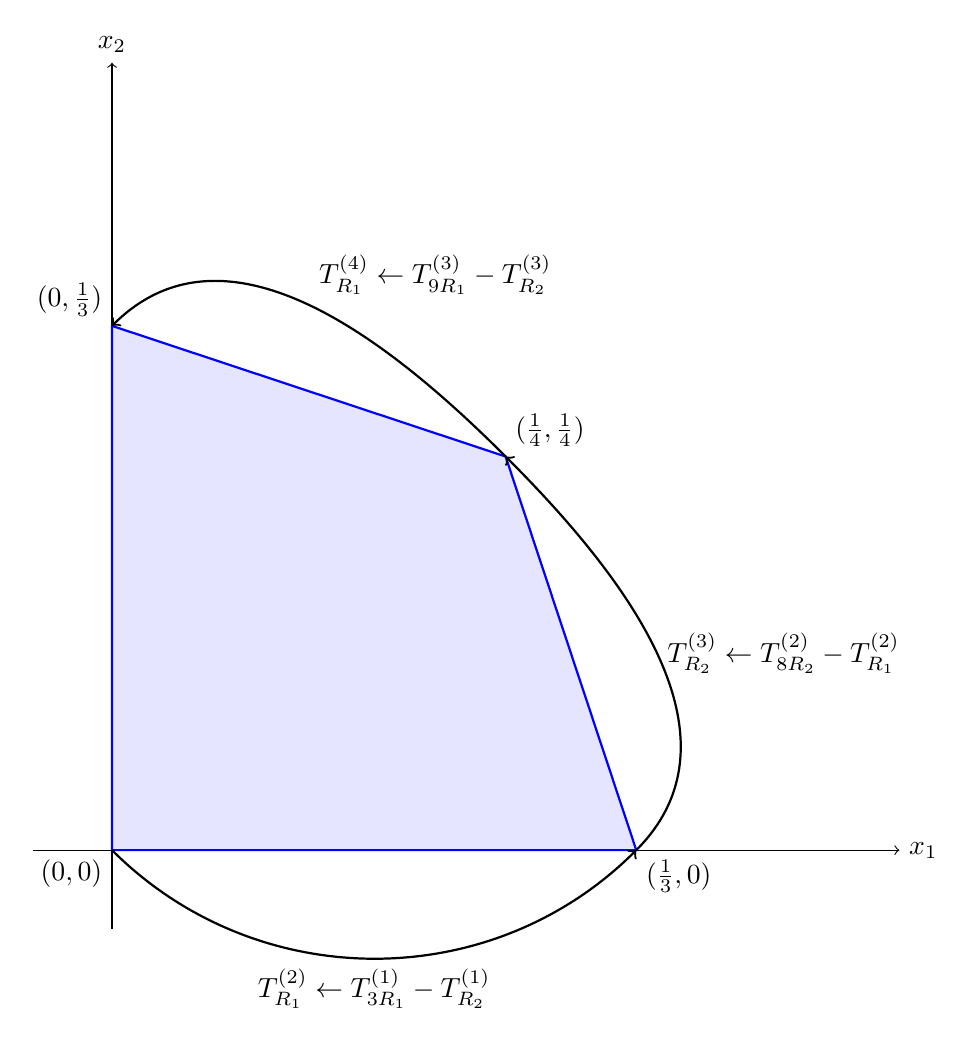
\begin{tikzpicture}[scale=20]
  % Ax_1es
  \draw[->] (-0.05, 0) -- (0.5, 0) node[right] {$x_1$};
  \draw[->] (0, -0.05) -- (0, 0.5) node[above] {$x_2$};

  % Define the points
  \coordinate (A) at (0, 0);
  \coordinate (B) at (0.333, 0);
  \coordinate (C) at (0.25, 0.25);
  \coordinate (D) at (0, 0.333);

  % Fill the polytope
  \filldraw[fill=blue!10, draw=blue, thick]
    (A) -- (B) -- (C) -- (D) -- cycle;


  % Label the points
  \node[below left] at (A) {$(0, 0)$};
  \node[below right] at (B) {$(\frac{1}{3}, 0)$};
  \node[above right] at (C) {$(\frac{1}{4}, \frac{1}{4})$};
  \node[above left] at (D) {$(0, \frac{1}{3})$};

  % Draw the pivoting steps
    \draw [->, thick] (A) to [out=-45, in=-135] node[midway, sloped, below]
    {$T^{(2)}_{R_{1}} \gets T^{(1)}_{3R_1} - T^{(1)}_{R_2}$}(B);

    \draw [->, thick] (B) to [out=45, in=-45] node[midway, right]
    {$T^{(3)}_{R_{2}} \gets T^{(2)}_{8R_2} - T^{(2)}_{R_1}$}(C);

    \draw [->, thick] (C) to [out=135, in=45] node[midway, above right]
    {$T^{(4)}_{R_{1}} \gets T^{(3)}_{9R_1} - T^{(3)}_{R_2}$}(D);
\end{tikzpicture}

\end{document}
